\documentclass{article}
\usepackage{graphicx}
\usepackage[margin=1.5cm]{geometry}
\usepackage{amsmath}

\begin{document}

\title{Thursday Reading Assessment: Chapter 7}
\author{Prof. Jordan C. Hanson}

\maketitle

\begin{figure}[ht]
\centering
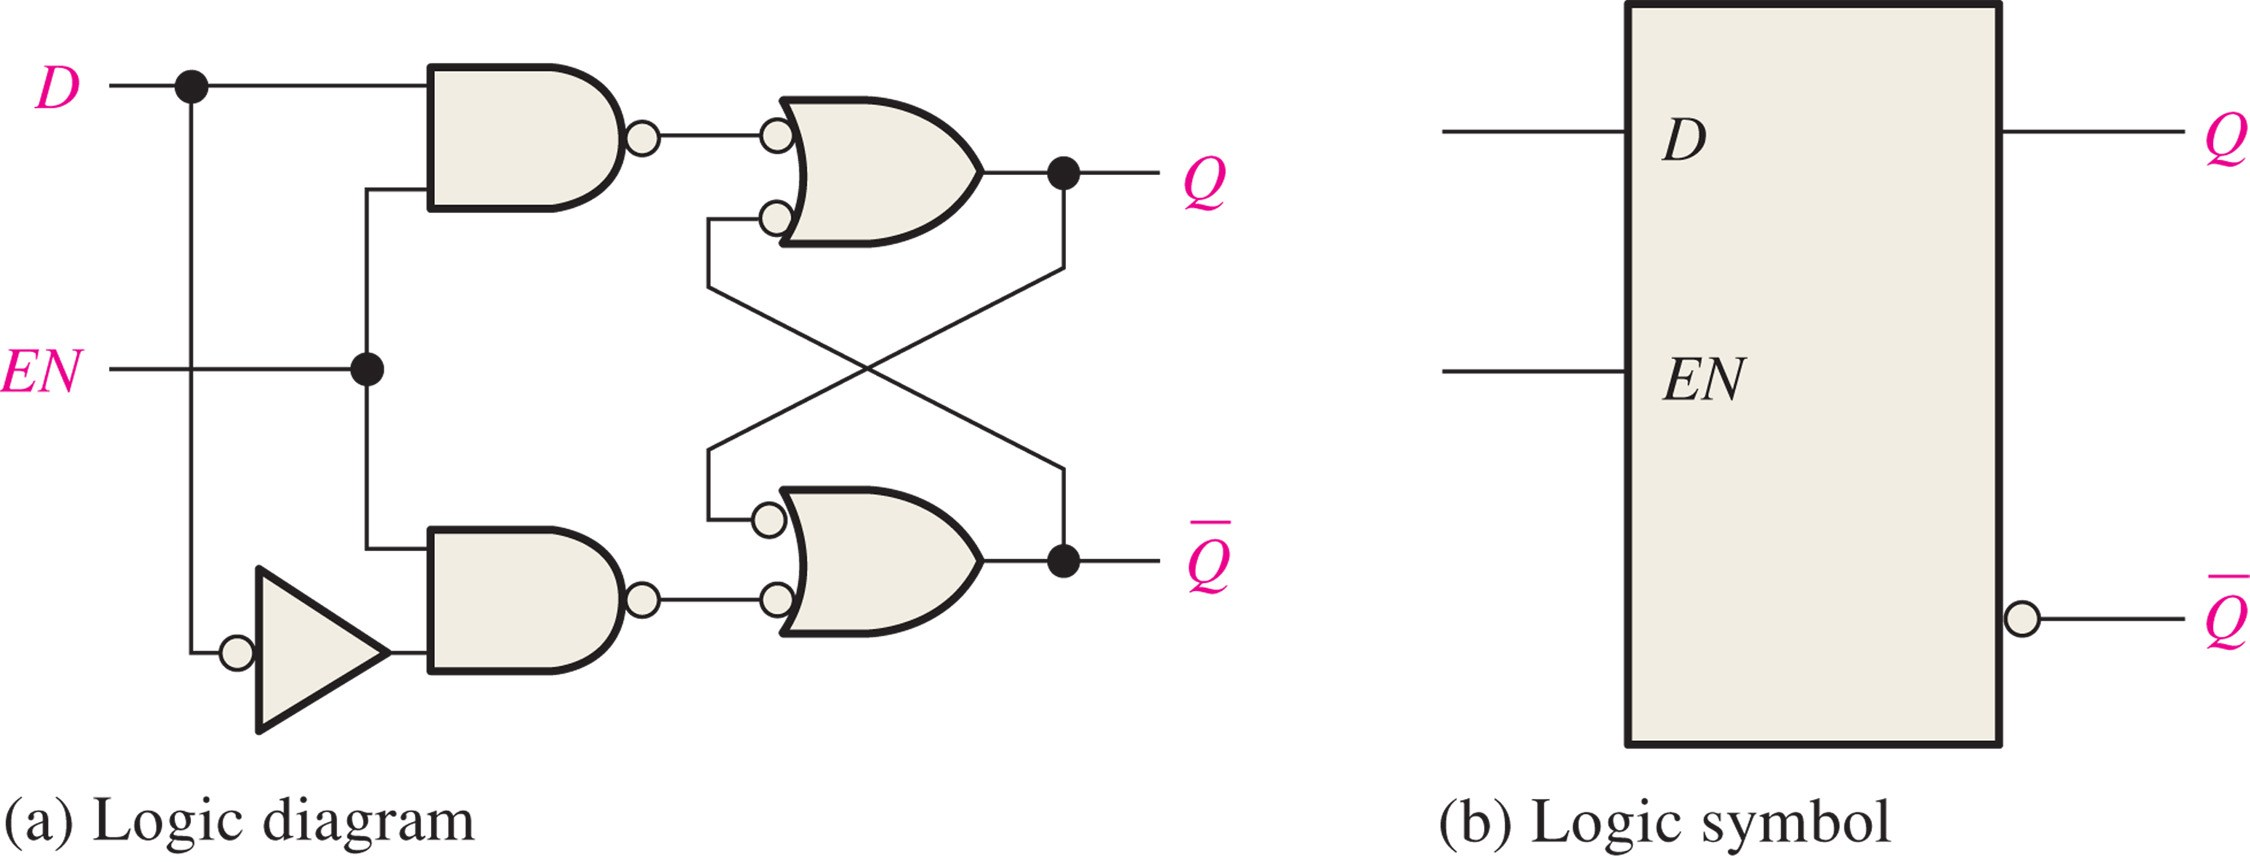
\includegraphics[width=0.4\textwidth,trim=0cm 1cm 0cm 0cm,clip=true]{figures/gated_D_latch.jpg} \hspace{0.1cm}
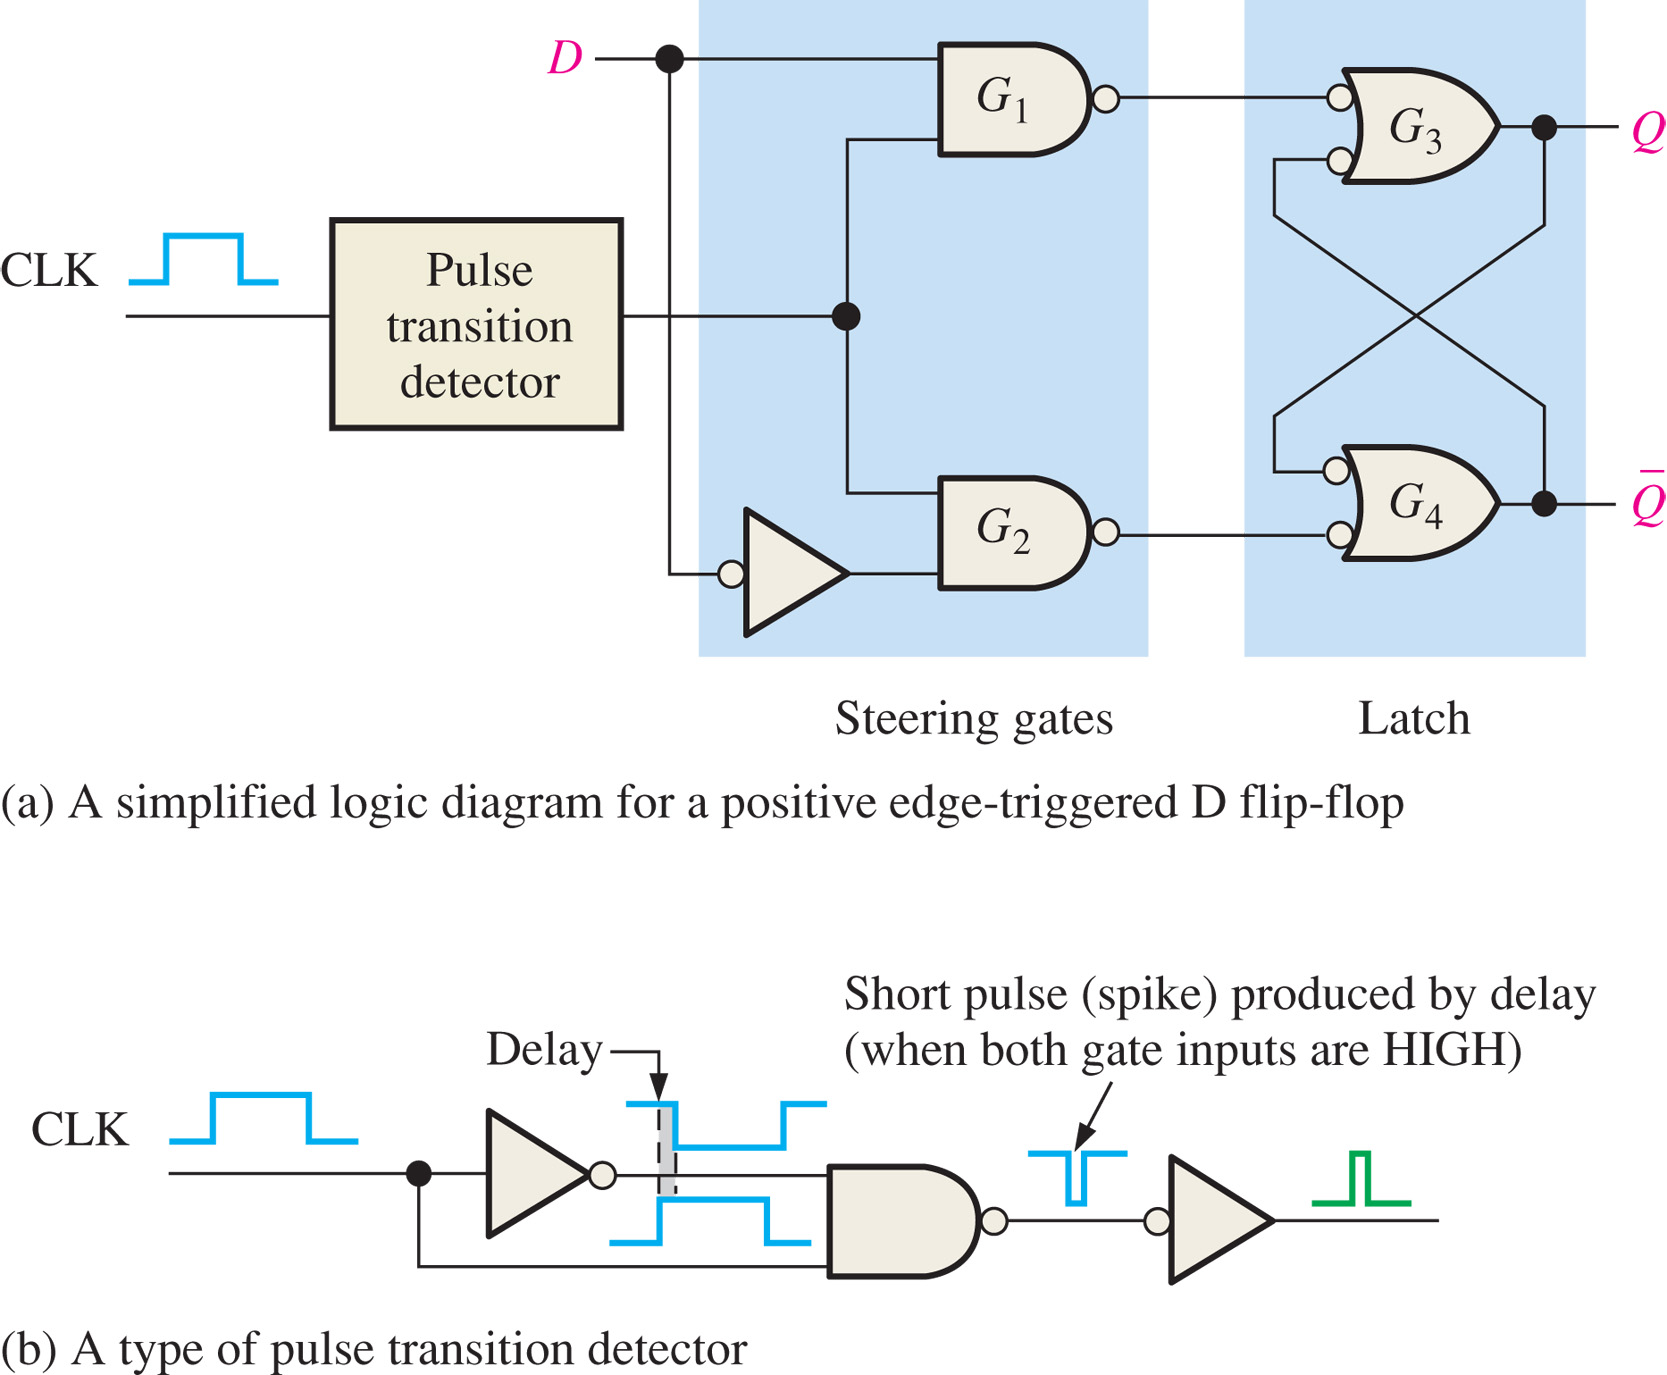
\includegraphics[width=0.4\textwidth,trim=0cm 0.5cm 0cm 9cm,clip=true]{figures/PTD.jpg}
\caption{\label{fig:1} (Left) A gated D-latch system expressed in terms of NAND gates. (Right) A pulse transition detector.}
\end{figure}

\section{Latches, Flip-Flops, and Timers: Gated D-latch}

\begin{enumerate}
\item (a) Produce the full truth table of the circuit in Fig. \ref{fig:1} (left) for the inputs $EN$ and $D$, and the outputs $Q$ and $\bar{Q}$. Remember to write $NC$ for ``No Change.'' (b) Create a timing diagram that enables the D-latch and passes the bitstream 10101010 from $D$ to $Q$, and then disables the D-latch.  What is the final state of the D-latch? \\ \vspace{2cm}
\end{enumerate}

\section{Latches, Flip-Flops, and Timers: Pulse Transition Detector}

\begin{enumerate}
\item (a) Produce the truth table for the \textbf{pulse transition detector} in Fig. \ref{fig:1} (right).  Assume the input states are constant values.  (b) If there is a 5 ns propagation delay in the initial inverter, what is the final pulse width?  (c) Introduce logic components to make the final pulse width 15 ns. \\ \vspace{2cm}
\end{enumerate}

\end{document}
